% !TEX root = ../main.tex

%************************************************
\chapter{SED Properties}
\label{ch:sed} 

% Refer to: 
% HotDustPaper/
 % summary-150309.ipynb
 % notes.md
 % correlations_summary_141204.ipynb
 % correlations_summary.md
 % various *.md 

%************************************************

\section{Introduction}

\begin{figure}
  \centering
  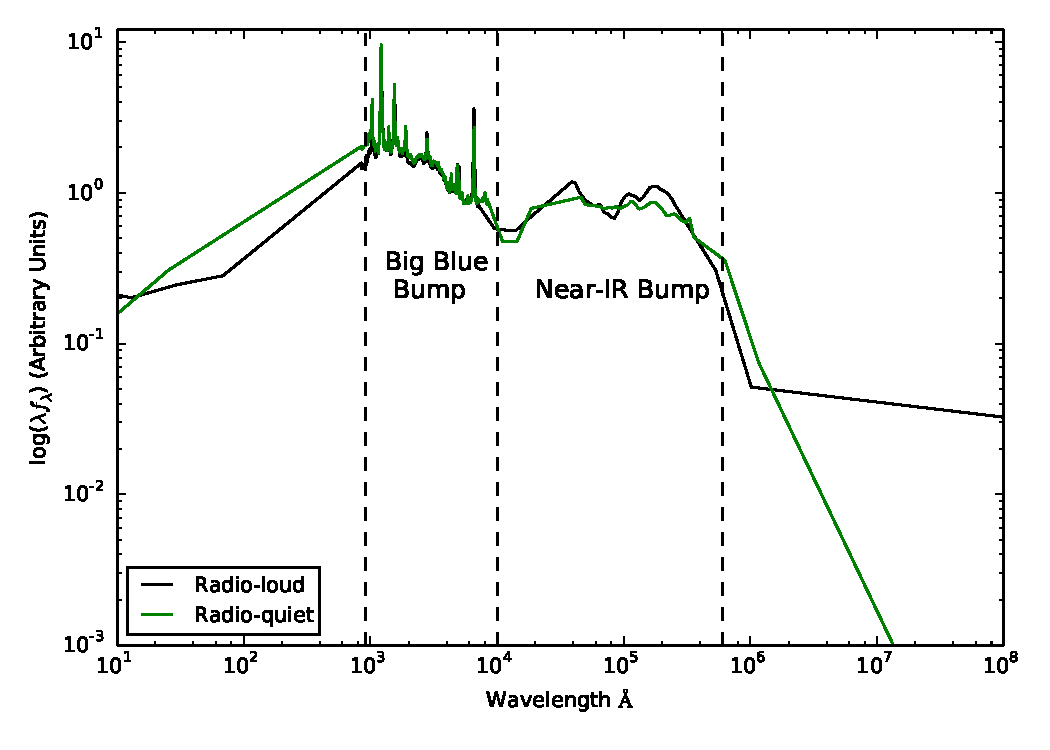
\includegraphics[width=\textwidth]{figures/chapter05/shangsed.pdf}
  \caption{Median radio-loud SED from \citet{shang11}.}
  \label{fig:seyfert_sed}
\end{figure}

AGN emit strongly over many decades in frequency (Figure~\ref{fig:seyfert_sed}). 
At different frequencies, the emission originates from processes occurring in different regions of the AGN. 
Hard X-ray emission is dominated by Compton up-scattering of accretion disk photons by electrons in a hot corona \citep[e.g.][]{sunyaev80}, UV/optical by thermal accretion disc emission, IR by dust at a wide range of temperatures, and radio by synchrotron emission in relativistic jets.   

Significant diversity is observed in the SEDs of individual objects. 
However, the systematic study of the dependence of the SED shape on physical parameters has, until very recently, been limited by the difficulty in obtaining a large sample of quasars with good multi-wavelength coverage and large dynamic range in luminosity and redshift. 
However, we are able to take advantage of a number of recent, sensitive, wide-field photometric surveys, including SDSS (in the UV/optical), UKIDSS (in the NIR) and WISE (in the mid-infrared).
We will combine this information with the BH mass and mass-normalised accretion rate estimates and outflow diagnostics which we developed in Chapters~\ref{ch:bhmass} and \ref{ch:nlr}. 
We will determine whether there are SED-related systematics as a function of outflow signatures and BH mass or Eddington ratio. 

Since the physical processes that power AGN are generally understood only qualitatively, almost all AGN SED templates are empirical. 
The empirical template of \citet{elvis94} is still the most commonly cited, despite many additions and updates \citep[e.g.][]{polletta00, kuraszkiewicz03, risaliti04, richards06,  polletta07, lusso10, shang11, marchese12, trichas12}. 
However, these composite spectra are often constructed from quasars with a huge range in luminosity as a function of wavelength. 
In addition, the presence of significant host galaxy at optical wavelengths in low-redshift objects is an additional complication which has not always been taken care of adequately. 
There is therefore a strong rationale for taking a parametric approach to modelling quasar SEDs. 
This is the approach we take in this chapter. 
We then investigate whether the systematic dependence of the model parameters on quasar properties including the BH mass, luminosity, accretion rate and outflow diagnostics. 

\subsection{Origin of hot dust emission}

Beyond some radius, this accretion disc is cool enough for dust accreting into it from the host interstellar medium not to be destroyed. 
If this dusty gas were ejected from the disk, it would be efficiently accelerated by the central continuum source because of the high cross section of dust. 
This would create a dusty wind from the disk. 
(Elitzur \& Ivezic 2001)

\section{Data}

\begin{table}
  \small
  \centering
  \begin{tabular}{lcccc}
    \hline 
    Survey & Band & $\lambda_{\mathrm eff}$ [$\mu{\mathrm m}$] & AB offset & $A_{\mathrm filter}/E(B-V)$ \\
    \hline 
    SDSS & $u$ & 0.3543 &  0.913 & 4.875 \\
         & $g$ & 0.4770 & -0.081 & 3.793 \\
         & $r$ & 0.6231 &  0.169 & 2.721 \\
         & $i$ & 0.7625 &  0.383 & 2.099 \\
         & $z$ & 0.9134 &  0.542 & 1.537 \\
    UKIDSS & $Y$ & 1.0305 &  0.641 & 1.194 \\
           & $J$ & 1.2483 &  0.941 & 0.880 \\
           & $H$ & 1.6313 &  1.378 & 0.569 \\
           & $K$ & 2.2010 &  1.897 & 0.352 \\
    WISE & $W1$ & 3.4 & 2.691 & 0.182\\
         & $W2$ & 4.6 & 3.331 & 0.130\\
         & $W3$ & 12.0 & & \\
         & $W4$ & 22.0 & & \\           
    \hline
  \end{tabular}
  \caption[{Available photometry, effective wavelength, Vega to AB magnitude offsets, conversion from $E(B-V)$ to extinction.}]{Available photometry, effective wavelength, Vega to AB magnitude offsets, conversino from $E(B-V)$ to extinction. \todoinline{Need W3/W4 offsets.}}
  \label{tab:photometry}
\end{table}

\subsection{SDSS DR7}

We use the Seventh Data Release (DR7) of the SDSS spectroscopic quasar catalogue \citep{schneider10}, which includes 105,783 objects across $\sim 9,380$ 9380 deg$^2$. 
The SDSS obtained images in five broad optical band-passes: $u$, $g$, $r$, $i$ and $z$ (Table~\ref{tab:photometry}).  
We use BEST point-spread function magnitudes.
Although the SDSS asinh magnitude system is intended to be on the AB system \citep{oke83}, the photometric zero-points are known to be slightly off the AB standard. 
According to the documentation\footnote{http://classic.sdss.org/dr7/algorithms/fluxcal.html}, the $u$ band zero-point is in error by 0.04 mag ($u_{\mathrm AB} = u_{\mathrm SDSS} - 0.04$) while the $z$ band is in error by 0.02 ($z_{\mathrm AB} = z_{\mathrm SDSS} + 0.02$). 
The $g$, $r$ and $i$ zero-points are consistent with the AB system. 

According to the online documentation\footnote{http://classic.sdss.org/dr4/algorithms/sdssUBVRITransform.html}, the magnitude of Vega in the SDSS magnitude system is $u=0.94$, $g=-0.08$, $r=0.17$, $i=0.40$ and $z=0.57$. 
Vega is estimated to have a magnitude $V=0.03$ in the Vega magnitude system. 
We use this information to estimate the zero-point offsets from the native SDSS magnitude system to the Vega system, given in Table~\ref{tab:photometry}. 
\todo{Update this once I confirm with Paul SDSS->AB->Vega conversions}

\subsection{UKIDSS Large Area Survey}

We use the tenth data release (DR10) of the UKIRT Infrared Deep Sky Survey \citep[UKIDSS;][]{lawrence07} Large Area Survey (ULAS) which has observed $\sim 3,200$ deg$^2$ in four NIR band-passes: $Y$, $J$, $H$ and $K$. 
We use `apermag3' magnitudes, which are aperture corrected magnitudes in a 2$''$ diameter aperture.
UKIDSS magnitudes are given in the Vega system. 
We adopt the Vega to AB zero-point offsets dervived by \citet{hewett06}; these are given in Table~\ref{tab:photometry}. 
\todo{Find out why Paul's AB offsets (given in the table) are slightly different.}

\subsection{WISE All-WISE Survey}

The Wide-field Infrared Explorer \citep[WISE;][]{wright10} mapped the entire sky in four mid-IR bands: $W1$, $W2$, $W3$ and $W4$. 
The WISE AllWISE Data Release (`AllWISE') combines data from the nine-month cryogenic phase of the mission that led to the `AllSky' data release with data from the NEOWISE program \citep{mainzer11}. 
We use the profile-fitting magnitudes (`w1mpro', 'w2mpro' etc.) 
WISE magnitudes are given in the Vega system, and Vega to AB conversion factors are given in the WISE Explanatory Supplement \citep{cutri13}.
\todo{Find out why Paul's AB offsets (given in the table) are slightly different.} 
\todo{Require S/N > 5?}

\subsection{Galactic extinction correction}

\todo{Confirm with Paul how this is calculated}
% The relative extinction between B and V bands E(B-V) at the position of each object are computed using the maps of \citet{schlegel98}. 
% Conversions from the selective extinction E(B-V) to the total extinction A in each band-pass were calculated by Paul, assuming a z=1.5 quasar spectral energy distribution and (I think) equation B2 in Schlegel+. 
% These are given in the table. 
% Do we also assume an extinction curve? 
% correcting for Galactic extinction using the maps of \citet{schlegel98}, assuming a Milky Way (MW) extinction curve \citep{pei92} and an extinction to reddening ratio ${\mathrm A}(V) / {\mathrm E}(B-V) = 3.1$. 

\subsection{Cross-matching}

Cross-matching the SDSS catalogue to the UKIDSS catalogue (with a 2$''$ matching radius) and to the WISE catalogue (with a 3$''$ matching radius) leaves 36,607 objects. 

We include only the ZZ quasars with $i$ band magnitudes brighter than 19.1, i.e. the quasars selected by the main SDSS quasar selection algorithm for quasars with colours consistent with being at redshifts $z < 3$ \citep{richards02}. 
Broad absorption line (BAL) quasars typically have redder spectra than non-BAL quasars. 
We therefore exclude these objects from our sample using the catalogue of BALs generated by \citet{allen11}. 
The redshift and luminosity distribution of the final sample, containing XX quasars, is shown in Figure~\ref{fig:lum_z}. 

\subsection{Completeness}

For a given $i$ magnitude, a quasar with a blue spectrum is more likely to be undetected at longer wavelengths than a quasar with a red spectrum. 
Therefore, as we allow fainter quasars into our sample we will be biased towards objects with redder spectra.
We verified that above the $i=19.1$ limit the sample is 95\% complete in all band-passes (excluding WISE $W3$ and $W4$).
\todo{This section needs clarification.} 

\begin{figure}
  \centering
  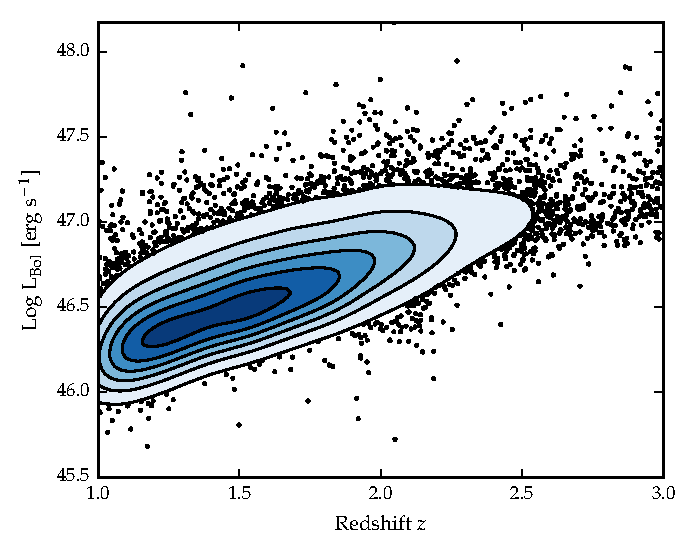
\includegraphics[width=\textwidth]{figures/chapter05/lum_z.pdf}
  \caption[{Distribution of our sample in the redshift-luminosity plane.}]{Distribution of our sample in the redshift-luminosity plane. \todoinline{Remake with new sample}}
  \label{fig:lum_z}
\end{figure}

% dr7dat.py 
% readdat.py
% DefingSample.ipynb 

\subsection{Generating the quasar catalogue}

\section{Quasar SED}

We have 19,853 quasars with photometric data from SDSS, UKIDSS and WISE. 
Our quasars cover the redshift range $0.2 < z < 4$, and so this data covers the rest-frame wavelength range from 800\AA\, to 3.8$\mu$m. 
In this region the SED is dominated by the accretion disc, emission lines and thermal emission from the hottest ($T\sim1200$K) dust. 
Host galaxy emission is also significant for quasars at redshifts $z\lesssim1$, and the effect of dust extinction at the AGN redshift is another factor which must be considered.   
In this section, we describe how we have modelled emission from these different physical processes. 
The model spectrum is shown in Figure \ref{fig:modelsed}, with each of the main components indicated. 

\section{SED Model}

\begin{figure}
  \centering
  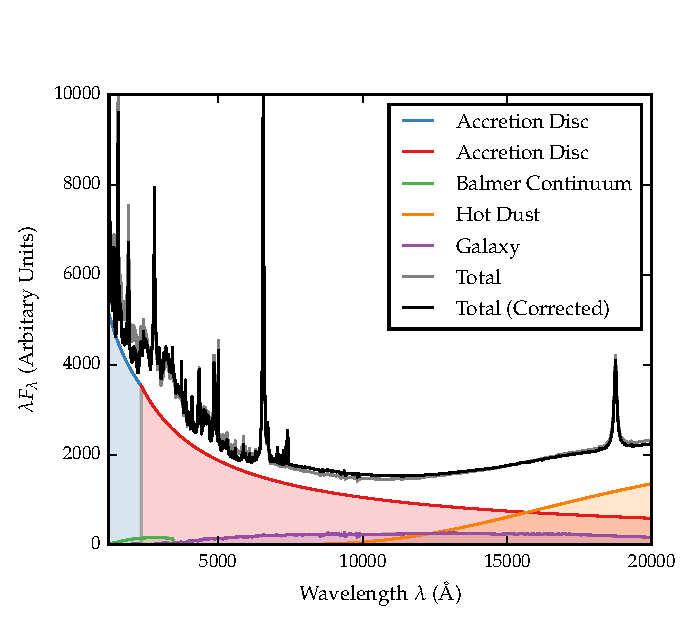
\includegraphics[width=\textwidth]{figures/chapter05/sed_model.pdf}
  \caption[{Model quasar spectrum at $z=1$, showing the contributions to the total flux from the blue power-law slope, red power-law slope, Balmer continuum, blackbody, emission line spectrum and host galaxy.}]{Model quasar spectrum at $z=1$, showing the contributions to the total flux from the blue power-law slope, red power-law slope, Balmer continuum, blackbody, emission line spectrum and host galaxy. \todoinline{Make sure it is immediately clear in every caption what is being shown in the figure.}}
  \label{fig:modelsed}
\end{figure}


\subsection{Accretion Disc}

Thermal accretion disc emission in the 0.1 - 1 $\mu$m region is characterised by a broken power-law with three free parameters: a break-wavelength $\lambda_{\mathrm break}$, a blue power-law index $\alpha_{\mathrm blue}$ for wavelengths shorter than the break wavelength, and a red power-law index $\alpha_{\mathrm red}$ for wavelengths longer than the break wavelength.

\subsection{Balmer Continuum}

High order Balmer lines, optically thin Balmer continuum emission, two-photon emission and \ion{Fe}{II} emission blend together to form a distinct feature in quasar spectra at $\sim3000$\AA. 
We simulate the Balmer continuum we use the empirical model given by \citet{grandi82}: 

\begin{equation}
  F(\lambda) = C_{\mathrm BC} \times B_\lambda(T_e)(1-e^{-\tau_\lambda}); \quad \lambda \leq \lambda_{\mathrm BE}
\end{equation}

where $C_{\mathrm BC}$ is a normalisation factor, $B_\lambda(T_e)$ is the Planck function, $T_e=13150$K is the effective temperature, $\lambda_{\mathrm BE}=3460$\AA\, is the wavelength at the Balmer edge, and $\tau_\lambda = \tau_{BE}\left( \nicefrac{\lambda_{BE}} {\lambda} \right)^{-3}$ is the optical depth with $\tau_{\mathrm BE}=45$ the optical depth at $\lambda_{\mathrm BE}$. 
This function is convolved with a Gaussian with $\sigma=5000$\kms to simulate the effect of bulk velocity shifts comparable to those present in broad AGN emission lines. 

\subsection{Hot Dust}

Thermal emission from hot dust, which dominates the SED at wavelengths longer than $1\mu$m, is modeled using a blackbody

\begin{eqnarray}  
  F_\lambda = C_{\mathrm BB} \times \frac{2 hc^2}{\lambda^5}\frac{1}{ e^{\frac{hc}{\lambda k_\mathrm{B}T_{\mathrm BB}}} - 1}, 
\end{eqnarray}

with two free parameters: the temperature $T_{\mathrm BB}$ and normalisation. 

\subsection{Emission Lines}

We use an emission line template taken from \citet{francis91}, which has been extended by \citet{maddox06} to include the \hans and Pa$\alpha$ emission lines \footnote{The spectrum is not significantly different from the \citet{vandenberk01} SDSS composite}. 
All emission lines, with the exception of \hans, are scaled using a single free parameter $C_{\mathrm EL}$, which preserves relative EQWs:

\begin{eqnarray}
  F_{\lambda} =  C_{\mathrm EL} \times \frac{F_{\lambda, \mathrm el}}{F_{\lambda, \mathrm cont}} \times F_{\lambda} ; \quad \lambda < 4700{\mathrm \AA} \;{\mathrm and}\; \lambda > 7000{\mathrm \AA} 
\end{eqnarray} 

where $F_{\lambda, \mathrm el}$ is the emission line template, $F_{\lambda,\mathrm cont}$ is the continuum flux in the template, and $F_{\lambda}$ is the continuum flux in the SED model.  
\hans, one of the strongest broad emission lines, is scaled separately: 

\begin{equation}
  F_{\lambda} =  C_{\mathrm EL} \times C_{{\mathrm H} \alpha} \times \left( \frac{L(z)} {L(z_{\mathrm nrm})} \right)^{-\beta} \times \frac{F_{\lambda, \mathrm el}}{F_{\lambda, \mathrm cont}} \times F_{\lambda}; \quad 4700{\mathrm \AA} < \lambda < 7000{\mathrm \AA} 
\end{equation}

The luminosity dependence of the \ha EQW (i.e. the Baldwin effect) is parametrised with a power-law with slope $\beta=0.04$.
The redshift dependence of the mean AGN luminosity $L(z)$ for the SDSS quasar catalogue has been determined empirically.

\subsection{Host Galaxy}

Emission from the host galaxy is important for AGN at redshifts $z\lesssim1$, particularly in the region around the $1\mu$m inflection point in the quasar SED. 
We use a $z=0$ Sb template from \citet{mannucci01}, which does not evolve with redshift.
The template is scaled by a multiplicative factor $C_{\mathrm Gal}$ and added to the AGN SED. 
We define a new parameter, $\eta$, the fractional contribution from the host galaxy to the total flux in the interval 4000 and 5000\AA:

\begin{eqnarray}
  \eta \equiv \frac{C_{\mathrm Gal}F_{\mathrm Gal}}{F_{\mathrm AGN} + C_{\mathrm Gal}F_{\mathrm Gal}},
\end{eqnarray}

where $F_{\mathrm Gal}$ and $F_{\mathrm AGN}$ are the flux of the galaxy and AGN respectively. 
Rearranging for the scaling factor $C_{\mathrm Gal}$ gives:

\begin{eqnarray}
  C_{\mathrm Gal} = \frac{\eta}{1 - \eta} \frac{F_{\mathrm AGN}}{F_{\mathrm Gal}}.
\end{eqnarray}

The fractional contribution to the total emission from the host galaxy decreases as the AGN luminosity increases and, in a flux-limited sample, the mean AGN luminosity increases as the redshift increases.
Therefore, the size of the host galaxy contibution to the SED is diminised for AGN at high redshifts ($z\gtrsim1$). 
At the same time, the shapes of the AGN and galaxy SEDs are very different. 
The galaxy SED peaks at $\sim1\mu$m, and falls away towards shorter wavelengths. 
On the other hand, the AGN SED continues to increase shortward of $1\mu$m. 
Therefore, the contrast between the AGN and galaxy luminosity increases as the redshift increases. 
We parametrize the AGN luminosity dependence of the host galaxy luminosity as a power-law:

\begin{eqnarray}
  \label{eq:lgal}
  \frac{L_{\mathrm Gal}}{L_{\mathrm AGN}} &=& L_{\mathrm AGN}^{\beta - 1} 
\end{eqnarray}

with slope $\beta=0.42$ \citep{croom04}. 
The galaxy scaling factor $C_{\mathrm Gal}$ becomes 

\begin{eqnarray}
  C_{\mathrm Gal} &=& \frac{\eta}{1 - \eta} \frac{F_{\mathrm AGN}}{F_{\mathrm Gal}} \left[ \frac{ L_{\mathrm Gal}(z)} {L_{\mathrm AGN}(z)} \right] \left[ \frac{ L_{\mathrm Gal}(z_{\mathrm nrm})} {L_{\mathrm AGN}(z_{\mathrm nrm})} \right]^{-1} \\
  &=& \frac{\eta}{1 - \eta} \frac{F_{\mathrm AGN}}{F_{\mathrm Gal}} \left[ \frac{L_{\mathrm AGN(z)}} {L_{\mathrm AGN(z_{\mathrm nrm}})} \right]^{\beta -1}, 
\end{eqnarray}

where $z_{\mathrm nrm}$ is an arbitrary redshift at which the fractional contribution from the host galaxy is by definition $\eta$. 

\subsection{Dust Extinction}
\label{sec:sed-extinction} 

The selection criteria of the SDSS DR7Q catalogue are sensitive to quasars with moderate amounts of dust reddening at the redshift of the quasar, and so we included the effect of dust extinction in our model. 
We use an extinction curve appropriate for the quasar population which has been derived by Paul Hewett. 
To derive the quasar extinction curve, UKIDSS photometry was used to provide an $E(B-V)$\footnote{$E(B-V)=A(B)-A(V)$} estimate, via the magnitude displacement of each quasar from the locus of un-reddened objects. 
At redshifts $2 < z < 3$ the reddening measure is made at rest-frame wavelengths 3500-7000\AA, where Galaxy, LMC and SMC extinction curves are very similar. 
The SDSS spectra of the same objects are then employed to generate an empirical extinction curve in the ultraviolet, down to 1200\AA. 
The resulting curve has no 2200\AA~ feature and rises rapidly with decreasing wavelength but is not as steep as the SMC curve. 
The extinctions curves give the colour excess $E(B-\lambda) = A$ relative to the colour excess $E(B-V)$ as a function of wavelength $\lambda$. 
The ratio of total to selective extinction, $R$, is defined as: 

colour excess $E(B-V)$ is related to the extinction in the $V$ band, $A(V)$, via the ratio  $R$, 

\begin{eqnarray}
  R_V = \frac{A(V)}{E(B-V)}
\end{eqnarray}

where we assume $R_V = 3$. 
Hence the extinction at a wavelength lambda $A(\lambda)$ is 

\begin{eqnarray}
  A(\lambda) = E(B-V) \times \left[ \frac{E(\lambda-V)}{E(B-V)} + R \right] 
\end{eqnarray}

where the colour excess $E(B-V)$ is a free parameter in our model. 
The attenuation of the flux at a given wavelength is then:

\begin{eqnarray}
  F_\lambda = F_\lambda10^{-A(\lambda)/2.5}
\end{eqnarray}

in the rest frame of the quasar. 

\subsection{Empirical Correction}

\todoinline{Describe Paul's empirical correction.}

\section{The `Standard' SED Model} 

\todoinline{
\begin{itemize}
    \item Given the same parameters, my model and Paul's look identical 
    \item I'm generating model colours using my model and Paul's best-fit parameters, and Paul's correction
    \item Do my model colours look the same as Paul's? (i.e. is there a bug in my code?)
    \item Can I generate the same median colours as Paul? (i.e. what sample is being used? what magnitudes?)
    \item Can I do my own fit to the data?  
\end{itemize}  
}

\begin{figure}
  \centering
  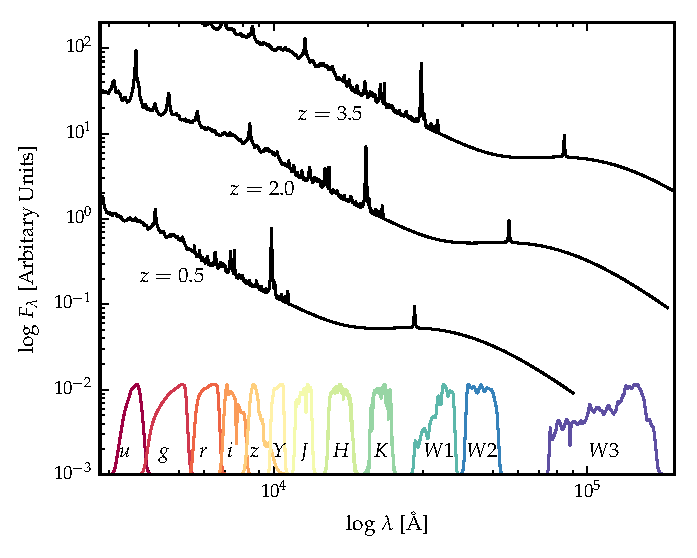
\includegraphics[width=\textwidth]{figures/chapter05/throughput.pdf}
  \caption[{Model quasar spectrum at three different redshifts, and throughput functions for SDSS, UKIDSS and WISE band-passes.}]{Model quasar spectrum at three different redshifts (each arbitrarily scaled), and throughput functions for SDSS, UKIDSS and WISE band-passes.}
  \label{fig:filters}
\end{figure}

We will begin by fitting a single SED model to all 19,853 quasars, encompassing a range of redshifts, luminosities, accretion rates etc. 
The free parameters in our model are the blue power-law slope, the red power-law slope, the power-law break wavelength, the blackbody temperature, the blackbody normalisation, the emission line EQW scaling, the \ha scaling and the fractional contribution from the host galaxy to the total flux. 
The reddening $E(B-V)$ is fixed to zero, since a large fraction of SDSS quasars have very small amounts of dust reddening \citep{richards03}. 
We generate a set of model observed spectra at redshifts from $z=0.25$ to $z=3.75$ in intervals of $\Delta z = 0.1$. 
The SED model is shown at three different redshifts in Figure~\ref{fig:filters}. 
The predicted broadband magnitude of the model is given by integrating the spectrum over the throughput for each of the bands.  

\begin{eqnarray}
  m_\lambda(P) & = & -2.5{\mathrm log}(f_\lambda(P)) - m_0(P), 
\end{eqnarray}

where $m_0(P)$ is the zero-point magnitude of band $P$ and the mean flux density $f_{\lambda}(P)$ is given by 

\begin{eqnarray}
  \label{eq:flux}
  f_{\lambda}(P) & = & \frac{\int P(\lambda) f_\lambda(\lambda) \lambda d\lambda }{\int P(\lambda) \lambda d\lambda}
\end{eqnarray}

where $P(\lambda)$ is the dimensionless throughput function of the band-pass. 
Magnitudes are calculated in the AB system (Oke \& Gunn 1983), in which case the zero-point flux per unit wavelength is 

\begin{eqnarray}
  \frac{f_\lambda(\lambda)}{{\mathrm erg}~{\mathrm cm}^{-2}~{\mathrm s}^{-1} {\mathrm\AA}^{-1}} = 0.1087 \left(\frac{\lambda}{\mathrm \AA}\right)^{-2}.
\end{eqnarray}


We divide our quasar sample into the same redshift bins.
In each bin we normalise the quasar SEDs in the SDSS $i$ band, and then calculate the median SED. 
The model SED in each redshift bin is similarly normalised. 
The chi-squared statistic is then minimised using the `nelder-mead' algorithm (\todoinline{reference}). 

Our SED model is valid only up to $\lambda \sim 3\mu$m in the quasar rest frame (the approximate wavelength of the peak in hot dust emission); beyond this additional contributions to the total flux from cooler dust will become significant. 
This prevents us from using the two longest wavelength WISE bands in the fit. 
We also exclude the SDSS $u$ and $g$ band-passes from the fit at $z > 2.7$ and $z > 3.7$ respectively, where these bands start to be affected by Ly$\alpha$ forest absorption.

\section{Results}

The best-fitting parameters from the fit are shown in Table \ref{tab:params}. 
\todo{Re-do fit}
The colours ($u - g$, $g - r$, etc.) of the median SED, the individual quasars, and the best-fitting model are plotted as a function of redshift in Figs.~\ref{fig:color_1} and \ref{fig:color_2}.
\todo{Need to show individual quasars.}  
Most of the large variations that can be seen in the median colours of the quasars as a function of redshift are due to strong emission lines being redshifted into and out of the band-passes.
Take away message is that a single, fairly simple parametric is able to reproduce the median colours of tens of thousands of AGN with a large dynamic range in redshift and luminosity. 
However, there is a significant scatter about the median model, which we will investigate in the next section?
Does any part of this scatter have a systematic dependence on properties of the BH (mass, accretion rate) or outflow diagnostics.  

\begin{table}
  \centering
  \begin{tabular}{c c c}
    \hline 
    Parameter & Symbol & Value \\
    \hline 
    Blue power-law index & $\alpha_{\mathrm blue}$ & 0.58 \\
    Red power-law index & $\alpha_{\mathrm red}$ & -0.04 \\
    Power-law break & $\lambda_{\mathrm break}$ & 2945 \\
    Blackbody temperature & $T_{\mathrm BB}$ & 1216 K \\
    Blackbody normalisation & $C_{\mathrm BB}$ & 0.22 \\
    Emission line scaling & $C_{\mathrm EL}$  & 0.63 \\
    \ha emission line scaling & $C_{{\mathrm H}\alpha}$  & 0.63 \\
    Galaxy fraction & $\eta$ & 0.29 \\
    \hline
    E(B-V) & E(B-V) & 0.00 \\
    \hline
  \end{tabular}
  \caption{Model parameters.}
  \label{tab:params}
\end{table}

\begin{figure}
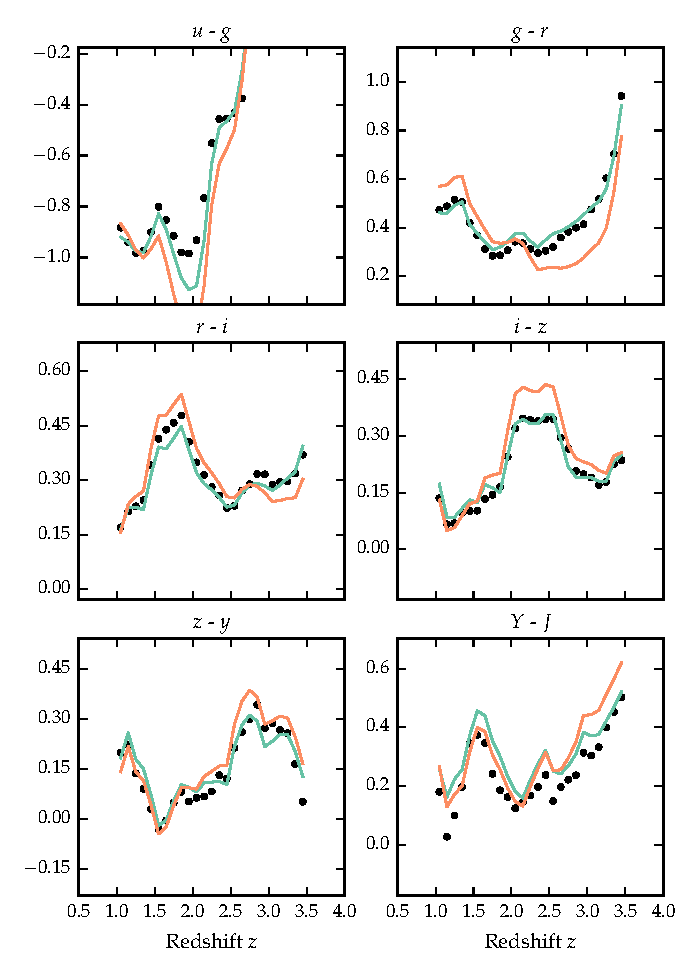
\includegraphics[width=\textwidth]{figures/chapter05/sed_color_plot_1.pdf}
\caption[{Colours of median quasar SED and best-fitting model, with and without correction.}]{Colours of median quasar SED and best-fitting model, with and without correction. \todoinline{Corrected is in orange, uncorrected in green. Check with Paul. Correction often makes colours a lot worse. Once got to the bottom of this just show with correction. Is Lyman forest absorption / lyman limit important for the quasars shown here.}}
  \label{fig:color_1}
\end{figure} 


\begin{figure}
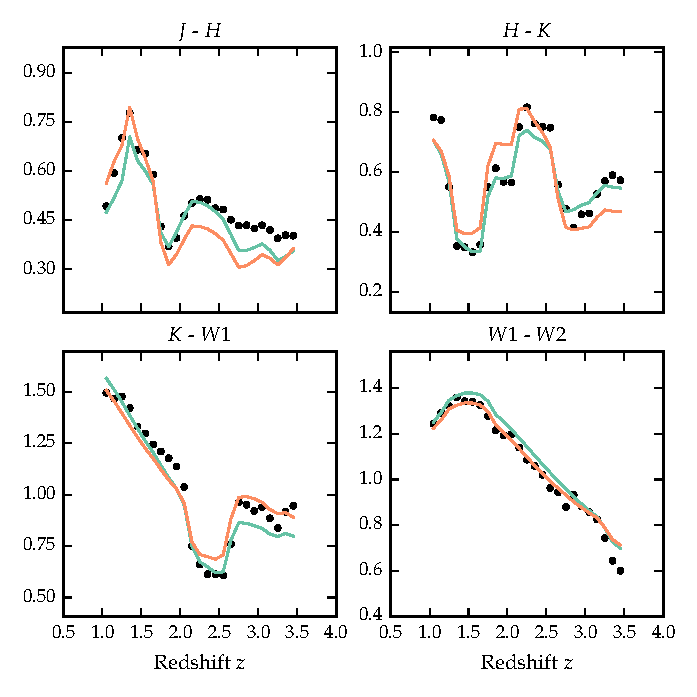
\includegraphics[width=\textwidth]{figures/chapter05/sed_color_plot_2.pdf}
\caption[{Colours of median quasar SED, individual objects, best-fitting  model as a function of redshift.}]{Colours of median quasar SED ({\it black circles}), individual objects ({\it grey points}), best-fitting  model ({\it black line}) as a function of redshift.}
  \label{fig:color_2}
\end{figure} 

\section{Discussion of Fit}

\begin{figure}
  \centering
  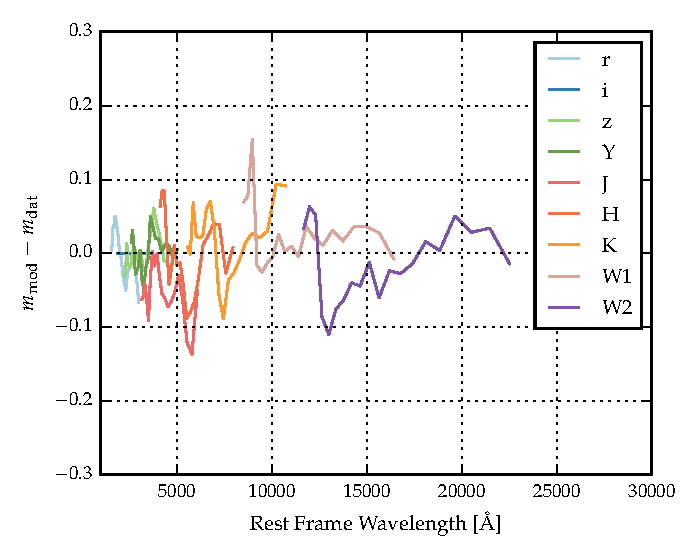
\includegraphics[width=\textwidth]{figures/chapter05/model_residuals.pdf}
  \caption[{Residuals from fit as a function of rest-frame wavelength.}]{Residuals from fit as a function of rest-frame wavelength. \todoinline{Need more info in caption.}}
  \label{fig:residuals}
\end{figure}

In Figure \ref{fig:residuals} we show the difference between the magnitudes from the best-fitting model and the median magnitudes from the sample. 
We have transformed the effective wavelengths of the band-passes to the rest frame of the quasars in each redshift bin, to give the residuals as a function of rest-frame wavelength. 
We represent the residuals measured in each band-pass using a different coloured line. 
Differences between residuals from different band-passes at the same rest-frame wavelength could indicate redshift evolution of the typical quasar SED. 

The residuals indicate that over a large redshift range the model does a fairly good at reproducing the median observed colours of the sample. 
\todo{No: be quantative}
Most discrepancies are at the $<0.1$ mag level. 
A single model is effective at reproducing the median colours, suggesting that the properties of a typical quasar do not change significantly over a wide range of redshifts and luminosities. 
\todo{Make sure this is emphasised as a new result.}
Many authors have found no significant dependence of the mean SED on properties such as redshift, bolometric luminosity, BH mass, or accretion rate \citep[e.g.][]{elvis12,hao13}. 
On the other hand, there is significant intra-sample variation. 
\todo{Need individual points on plot to show this.} 

\section{Hot Dust}

\begin{figure}
\centering
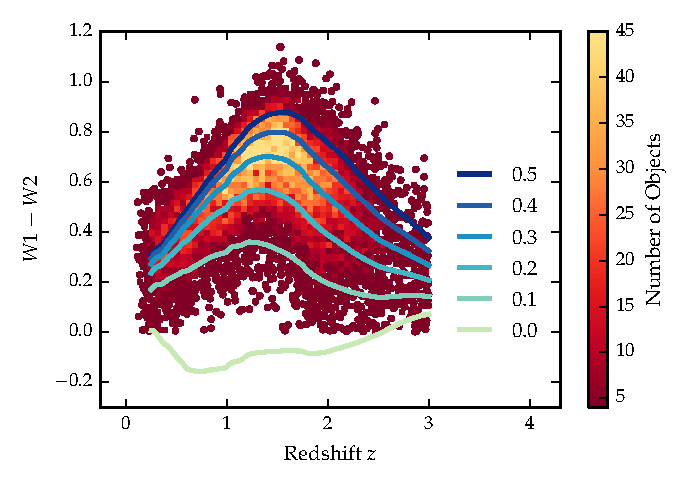
\includegraphics[width=\columnwidth]{figures/chapter05/w1w2_versus_redshift_ratio.pdf}
\caption[{$W1 - W2$ colours of sample as a function of redshift.}]{$W1 - W2$ colours of sample as a function of redshift. Above a certain density threshold points are represented by a density plot. On top we plot the colours of our standard SED model, with a fixed temperature and a varying NIR (1 - 3 $\mu$m) to UV ratio.}
  \label{fig:w1w2colorsratio}
\end{figure}

The spread in the $KW1W2$ colours (Figure~\ref{fig:w1w2colorsratio}), probing the rest-frame $\sim$1-2 micron region, is significant and strongly suggests the presence of real variation in the hot dust temperature and luminosity among the quasars. 

\subsection{Parametrising the hot dust emission}

We characterise the hot dust properties of our sample in terms of the temperature and luminosity of a blackbody.  
We choose to parametrise the luminosity in terms of the NIR to UV luminosity ratio (which is proportional to the covering factor of hot dust ($L_{NIR}/L_{Bol}$) used in other studies \citep{roseboom13}. 
The UV and NIR luminosity are calculated between 2000 and 9000\AA\, and 1 and 3 $\mu$m respectively.

If the hot dust emission is dominated by emission from the inner edge of a torus, then the temperature is related to the distance from the dust to the central source. 
If the inner edge of the torus is further from the accretion disc, then the dust will be cooler.
If instead the dust is in an outflows, then the interpretation of the dust temperature is less clear.  
The value of ($L_{NIR}/L_{Bol}$) is related to the covering factor of the hot dust. 

Some previous studies \citep[e.g.][]{wang13,zhang14} have instead parametrised the NIR emission using a power-law ($\propto \lambda^{\beta_{\mathrm NIR}}$), with $\beta \simeq 0.5$. 
We tested this parametrisation, and evaluated it's effectiveness relative to using a blackbody. 
We normalise the power-law at 9000\AA, where its flux is set equal to the flux of the UV/optical model. 
The NIR power-law slope is fit between $\sim$1 and 2.4$\mu$m (with the exact wavelength region being fit depending on the redshift of the quasar). 
We found large residuals in the best-fitting model which varied systematically as a function of $\lambda_{eff}/(1+z)$.  
This suggests that the power-law model is a poor fit to the shape of the NIR emission. 
One needs to take care in looking at trends with luminosity given the observed-frame band-pass information on the rest-frame SED can produce some strong systematics with redshift, particularly if the SED-model is not a good fit to the actual SED. 
A similar conclusion was reached by \citet{gallagher07}.

\subsection{Sample}

Our goal is to determine the temperature and abundance of the hot dust component in individual quasars.  
These properties will be measured by fitting a model to the SDSS-UKIDSS-WISE photometry. 
Constraining a T$\sim$1200K blackbody component in the SED model requires photometric data covering $\sim$1-3$\mu$m in the rest-frame of the quasar. 

The observed-frame wavelength coverage of the available band-pass limits the redshift range of the quasars which can be used. 
We consider only quasars at redshifts $z>1$ where the relative host galaxy contribution to the SED is negligible. 
At redshifts $1 \lesssim z \lesssim 1.5$ the available $ugrizYJHKW1W2$ photometry provides good coverage of the rest-frame SED up to $\sim$2$\mu$m.
At $z\sim1.5$ the W2 band-pass is shifted to $\sim$1.8$\mu$m; at higher redshifts W2 is probing much shorter wavelengths than the peak of a T$\sim$1200K blackbody. 
Because the shape of the blackbody is not well constrained by the available photometry, the uncertainty on the blackbody temperature measurement increases sharply for quasars at redshifts $z\gtrsim1.5$ 

For the quasars at $z \sim 1$, the WISE W3 band is probing rest-frame wavelengths of $\sim5-6\mu$m. 
This region of the SED is dominated by emission from cooler, more distant dust, which is not accounted for in our model.
However, at redshifts $z \gtrsim 2$ the WISE W3 band-pass probes sufficiently short wavelengths to be useful in constraining the shape of the hot blackbody component. 
Therefore, for quasars at redshifts $z > 2$ we again have sufficient constraints from the $ugrizYJHKW1W2W3$ photometry to determine the temperature and normalisation of the blackbody component. 
There are few objects in our sample with redshifts $z > 2.7$, because the SDSS DR7 quasar selection algorithm is highly incomplete at these redshifts.  
Therefore we set $z=2.7$ as the upper limit on the redshift of our sample. 
Because of these constraints, our sample is divided into two parts: one at low redshifts ($1 < z < 1.5$) and the other at higher redshifts ($2 < z < 2.7$). 

We impose a lower-limit signal-to-noise ratio (S/N) $>$ 5 magnitudes in the $K$, $W1$ and $W2$ band-passes for the low-$z$ sample and S/N > 5 in the $W1$, $W2$, and $W3$ band-passes for the high-$z$ sample to ensure reliable photometry.
This gives us 5,910 quasars in our low-$z$ sample and 1,989 quasars in our high-$z$ sample. 

\begin{table}
  \small
  \centering
  \begin{tabular}{cccc}
    \hline 
    Sub-sample & Number of AGN & Data & Redshift range \\
    \hline 
    Low-$z$ & 5,910 & $ugrizYJHKW1W2$ & $1 < z < 1.5$ \\
    High-$z$ & 1,989 & $ugrizYJHKW1W2W3$ & $2 < z < 2.7$ \\           
    \hline
  \end{tabular}
  \caption{Summary of sub-samples.}
  \label{tab:sub-samples}
\end{table}


We will hold most model parameters fixed, and vary only the blackbody parameters which parametrise the NIR emission. 
Therefore, we need to define a sub-sample of objects which we know are well fit by our standard SED model in the UV/optical region. 
This means excluding objects with extreme emission line EQWs and/or significant dust extinction.
We use the $i-K$ colours of the quasars as a measure of the overall colour of the quasars as it provides the longest baseline in wavelength without being affected by absorption in the Ly$\alpha$ forest at high redshifts. 
A significant amount of the scatter in $i-K$ can be attributed to intrinsic variations in the UV power-law slopes of the individual quasars, which is why we allow a negative reddening. 
However, there is a clear `red tail' to the colour distribution which can be explained by dust reddening at the redshift of the quasar.
We discarded from our sample quasars with $i - K$ colours redder than our standard model with dust reddening E(B-V) = 0.075 and bluer than E(B-V) = -0.075 (Figure~\ref{fig:ikzplot}). 
Following this cut we are left with 4,615 quasars in our low-$z$ sample and 1,692 quasars in our high-$z$ sample. 

The SDSS and UKIDSS photometry are separated by 3-4 years in the source rest-frame. 
Therefore, some of the $i-K$ scatter could be due to temporal variations in the brightness of the targets. 
However, the red-asymmetry of the $i-K$ colours about the un-reddened SED model suggests that this effect is sub-dominant to intrinsic colour differences. 

\begin{figure}
  \centering
  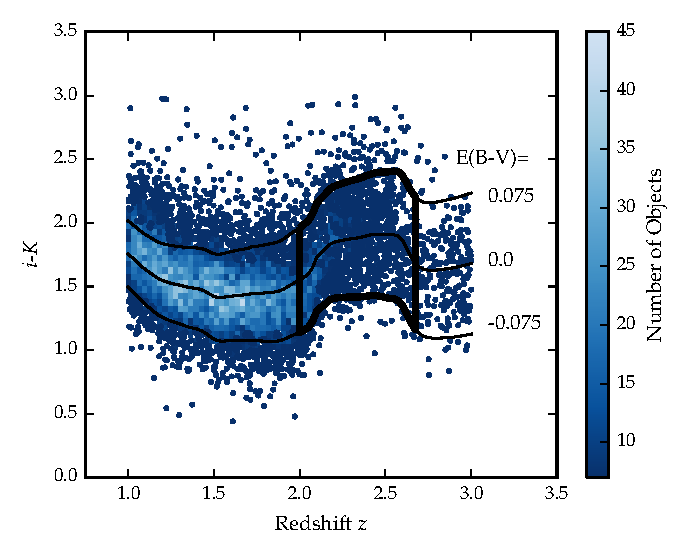
\includegraphics[width=\columnwidth]{figures/chapter05/ik_versus_z_low_ext.pdf}
  \caption[{$i-K$ colours of non-BALQSO DR7Q quasars with $i>19.1$ as a function of redshift.}]{$i-K$ colours of non-BALQSO DR7Q quasars with $i>19.1$ as a function of redshift. The lines show the colours of our model with varying amounts of dust extinction. Quasars with extinction $|E(B-V)|>0.075$ are excluded.}
  \label{fig:ikzplot}
\end{figure}

\subsection{Diversity in hot dust properties}

In Figure~\ref{fig:w1w2colorsratio} we plot the $W1 - W2$ colours of the sample as a function of redshift at $z<3$. 
In this redshift range the $W1$ and $W2$ band-passes are probing the 1.2 - 2.8$\mu$m and 1.6 - 3.8 $\mu$m region of the rest frame SED respectively. 
For reference, the peak wavelength is at 2.4$\mu$m for a blackbody radiating at 1200K. 
At any given redshift we see a $\sim 0.5$ mag dispersion in the $W1-W2$ colours. 

On the same axes in Figure~\ref{fig:w1w2colorsratio} we have plotted the $W1-W2$ colours derived from our SED model with a fixed blackbody temperature (1216K) and a ratio of NIR to UV luminosity ranging from 0.0 to 1.0, with the other model parameters held constant. 
We conclude that even with the sample restricted to be uniform in its UV/optical properties, we still get an significant spread in $W1-W2$ colours, which we can use to learn about the diversity of NIR properties in our sample. 
In the rest of this chapter we will characterise the hot dust properties of our sample, and test its relation to quasar properties such as luminosity, black-hole mass and normalised accretion rate, and outflow-properties. 

\section{Fitting procedure}

We will fit a model to the individual quasar SEDs, allowing the temperature and normalisation of the black body component to vary. 
The model spectrum is redshifted to the redshift of the quasar being fit and is then multiplied by the $ugrizYJHMW1W2W3$ throughput functions and normalised appropriately to give AB magnitudes. 
We minimise the chi-squared statistic using the minimisation is done using the 'nelder-mead' algorithm.
To avoid significant absorption in the Ly$\alpha$ forest at high-$z$, we restrict our fitting to wavelengths greater than 2000A; when the effective wavelength of a band-pass falls below this limit the band-pass is excluded from the fit. 
\todo{2000A is quite large given the Ly-alpha forest impacts from 1216A.}
$W3$ is only used for the quasars at redshifts $2 < z < 2.7$. 

\section{Results}

\todo{Show some example fits? Show overlayed data/model with alpha=0.1?}

In Figure~\ref{fig:ratio_tbb_density} we see that the two parameters are clearly correlated. 
For a lower temperature blackbody the NIR to UV luminosity ratio is larger. 
Such a correlation is to be expected: as the blackbody temperature is lowered, the peak shifts to longer-wavelengths (following Wien's displacement law). 
Because of this degeneracy we need to be very careful to separate out real trends of $R_{NIR/UV}$ with other quasar properties from indirect trends resulting from a mutual dependence on $T_{BB}$.  

\begin{figure}
  \centering
  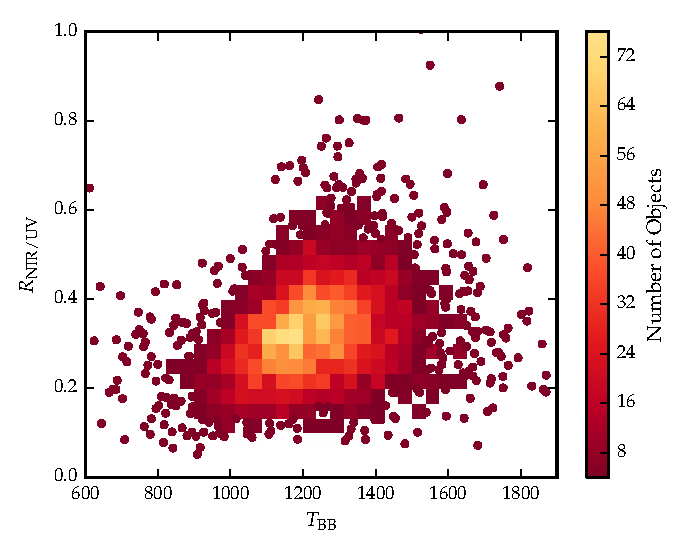
\includegraphics[width=\textwidth]{figures/chapter05/ratio_tbb_density.pdf}
  \caption[{Ratio of NIR to UV luminosity ($R_{NIR/UV}$) against temperature ($T_{BB}$) for low-$z$ sample.}]{Ratio of NIR to UV luminosity ($R_{NIR/UV}$) against temperature ($T_{BB}$) for low-$z$ sample. The density of points is shown in more dense regions of the space, and individual objects in less dense regions. }
  \label{fig:ratio_tbb_density}
\end{figure}

In Figure~\ref{fig:ratio_tbb_density} we show that there is significant range of temperature and normalisation present in our sample. 
However, we need to quantify  how much of this is due simply to uncertainties in the fits stemming from uncertainties in the photometry. 
In order to achieve this we took our standard SED model with a single temperature and normalisation blackbody component, and generated 200 mock SEDs with a brightness distribution similar to that of our real sample. 
We estimated the mean uncertainty of the magnitudes in the $K$, $W1$, and $W2$ band-passes as a function of apparent brightness. 
We then sampled the $K$, $W1$, and $W2$ magnitudes from Gaussian distributions, with a mean equal to the magnitude of the model SED, and the width equal to the mean uncertainty at the appropriate brightness. 
Finally, we fit these mock SEDs using our standard fitting procedure. 
The results are shown in the Figure below, on top of the results from our real sample (shown as grey contours). 
We can see that uncertainty in the photometry introduces a significant scatter to the temperature, but that this scatter is significantly less than the intrinsic scatter in the data. 
This demonstrates that there is a real distribution of hot dust temperatures and luminosities in our sample. 

\begin{figure}
  \centering
  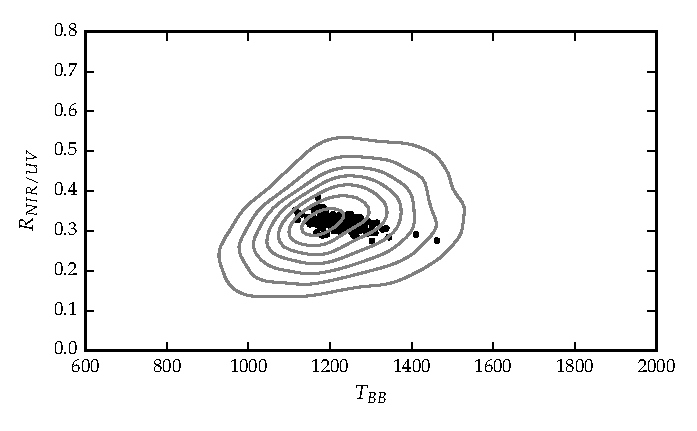
\includegraphics[width=\textwidth]{figures/chapter05/ratio_tbb_contours.pdf}
  \caption[{Ratio of NIR to UV luminosity ($R_{NIR/UV}$) against temperature ($T_{BB}$).}]{Ratio of NIR to UV luminosity ($R_{NIR/UV}$) against temperature ($T_{BB}$). The grey contours show equally-spaced lines of constant probability density generated using a Gaussian kernel-density estimator on our data sample. The black points are for our mock data.}
  \label{fig:ratio_tbb_contours}
\end{figure}

\subsection{Correlations with quasar properties}

\begin{figure}
  \centering
  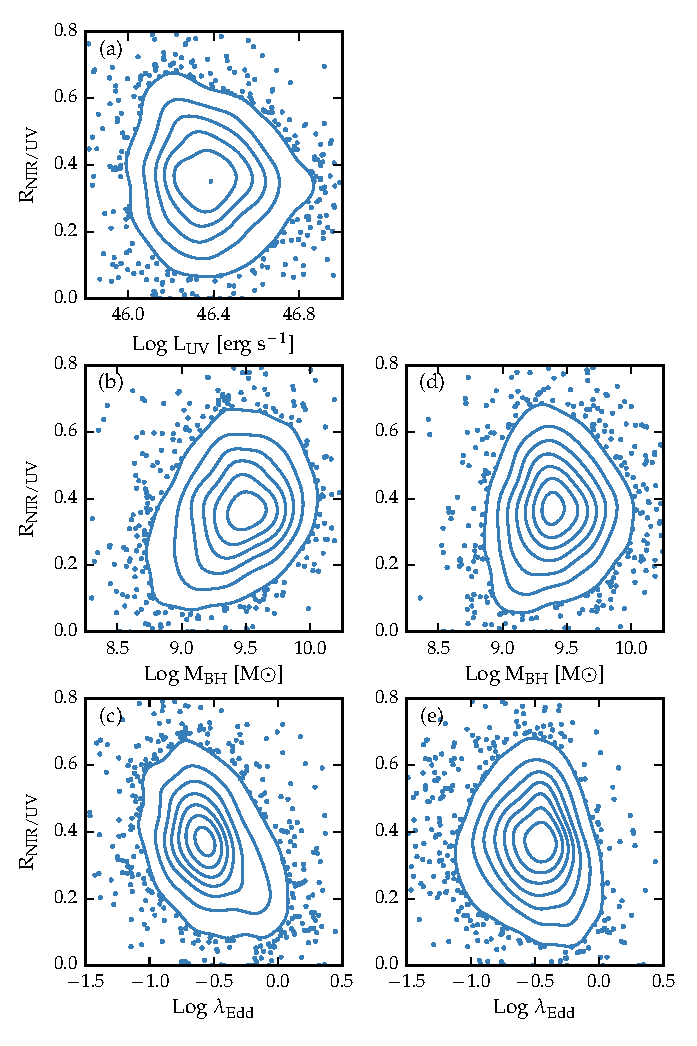
\includegraphics[width=\textwidth]{figures/chapter05/correlations_contour.pdf}
  \caption[{Best-fit blackbody temperature against UV luminosity, black-hole mass and Eddington ratio.}]{Best-fit blackbody temperature against UV luminosity (left), black-hole mass (centre) and Eddington ratio (right) for $1 < z < 1.5$ sample (black) and $2 < z < 2.7$ sample (black). In region of high-density we represent the density with contours generated using a Gaussian kernel density estimation. \todoinline{Needs re-making with new BH masses.} \todoinline{Maybe just show as one sample?}}
  \label{fig:correlations_contour}
\end{figure}

We now look for correlations between the properties of the blackbodies we have fitted to the hot dust emission and other properties of the quasar such as redshift, BH mass, normalised accretion rate (Eddington ratio), and outflow diagnostics.  
\todo{Calculate new BH masses and redo this section.}

% There is a clear anti-correlation between the UV luminosity and the best-fit blackbody temperature. 
% We calculated a Spearman rank-order correlation coefficient -0.33. 
% \todo{Do we believe this trend is real?}
% \todo{This is just for low-z sample.}
% The black-hole masses are virial estimates calculated by Shen et al. 2011 using the MgII emission line in the SDSS spectra. 
% The Eddington ratios (bolometric luminosity normalised by Eddington luminosity) are also calculated by Shen et al. 2011 using bolometric corrections in Richards et al. (2006a) using 3000\AA monochromatic luminosities. 
% There are no significant correlations between $T_BB$ and $R_{NIR/UV}$ and the UV luminosity, black-hole mass or Eddington ratio. 

% The dynamic range in luminosity is very limited. 
% I will combine the low and high $z$ samples. 
% As first step see if there is a difference in the median $R_{NIR/UV}$ for low/high luminosity samples. 

% At low-$z$  we get a much larger range in blackbody temperatures from our fits. 
% We discussed how the W3 S/N > 5 cut might be be biasing the high-z sample if the subset being removed had properties distinct from the remainder of the sample. 
% The W3 S/N > 5 cut removes about 25\% of the sample. 

% We observe a postive correlation between the black-hole mass and the NIR to UV luminosity ratio which is quite different from what we observed in our low-$z$ sample. 
% We believe that this is just a manifestation of the fact that at high redshift the black-hole masses are derived from CIV. 
% We will show below how the FWHM of CIV has a positive correlation with the hot dust abundance, and large CIV FWHM leads to larger black hole mass estimates. 
% This explains the apparent correlation between the IR/UV ratio and the black hole mass. 
% Eddington ratio measures the luminosity relative to the Eddington luminosity. 
% Higher blackhole mass estimates will lead to lower Eddington ratios, which is why the Eddington ratio appears to decrease with increasing IR/UV ratio. 
% For the sources in our low-$z$ sample the black-hole mass is measured using the broad MgII emission line. 
% As we will show below, the properties of the MgII emission line have no dependence on the hot dust properties. 


\subsubsection{Composite spectra}

\begin{figure}
  \centering
  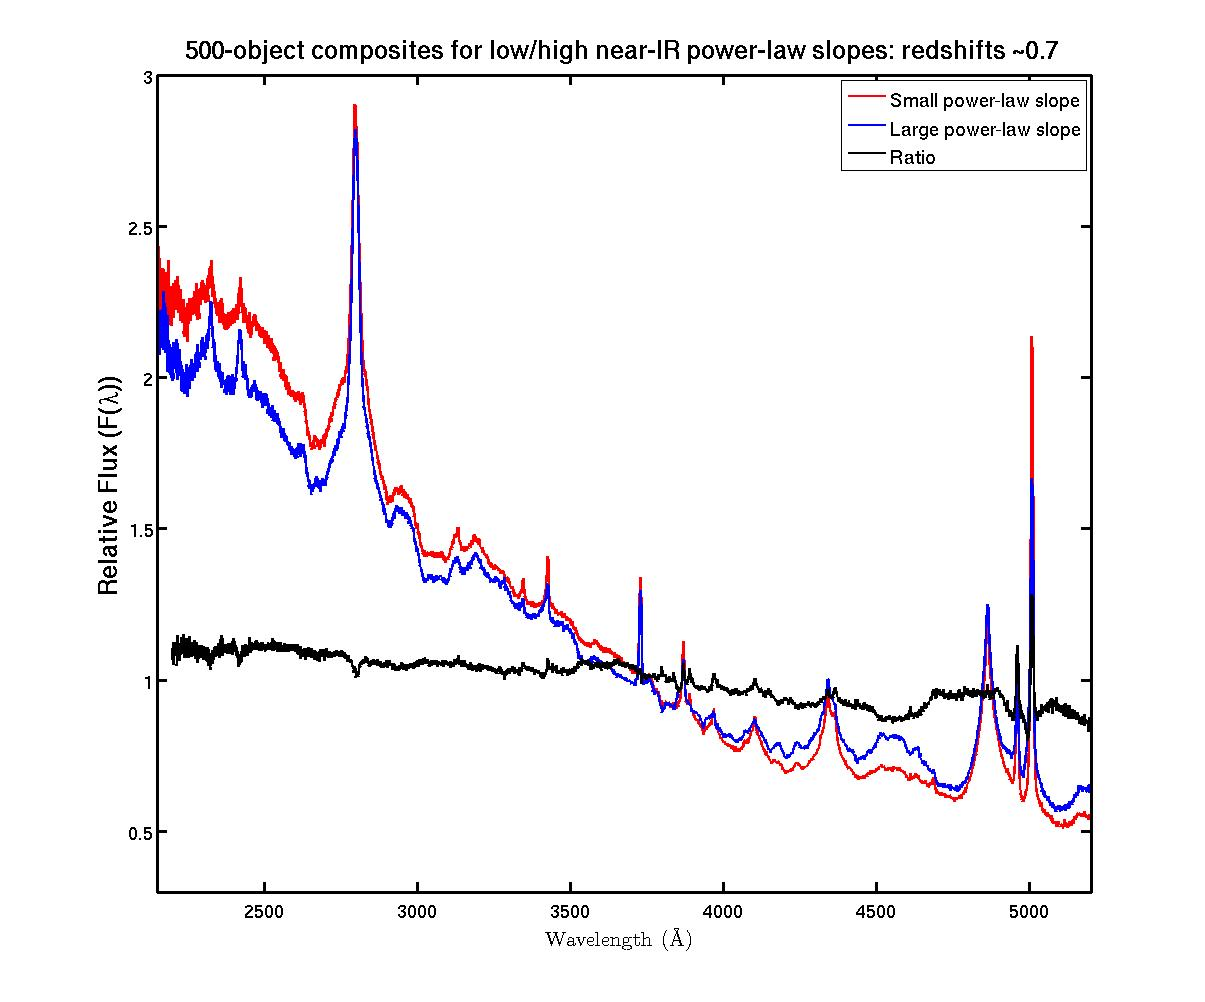
\includegraphics[width=\textwidth]{figures/chapter05/z07_pls_comps.jpg}
  \caption[{Composite SDSS spectra for objects at $z\sim0.7$.}]{Composite SDSS spectra for objects at $z\sim0.7$. We have divided sample into objects with objects best-fit by small (red line) and large (red line) values of $\beta$. \todoinline{Remake if possible}.}
  \label{fig:pls_comp}
\end{figure}

Is there a connection between the hot dust properties and EV1? 
To test this we can divide the quasar sample by hot dust properties, and then generate composite spectra. 
The EV1 original EV1 correlates - \ion{Fe}{II}, \hb, [\ion{O}{III}] - are at around 4000-6000\AA. 
The SDSS spectra are probing shorter wavelengths at redshifts $z\gtrsim1$.
Recall that our sample does not include any quasars at redshifts $z<1$, where the host galaxy emission starts to become significant. 
\todo{Need to decide what to do here. If I say host galaxy is significant using the power-law slope won't help. Use blackbody fits instead?}

The $z < 0.8$ SDSS spectrum composite comparison for the small and large $\beta_{NIR}$ sub-samples (Figure~\ref{fig:pls_somp}) is a very direct illustration of EV1. 
Hot dust emission increases with \ion{Fe}{II} EW. 
We also note that the amount of hot dust correlates with the \ion{Si}{III}/\ion{C}{III}] emission ratios. 
The \ion{Si}{III}/\ion{C}{III}] ratio is generally considered to be a good indicator of density and is one of the primary EV1 correlates. 
The relative flux ratio of \ion{Si}{III} to \ion{C}{III}] increases when \ion{C}{IV} is more blue-shifted \citep{richards11}. 
The \ion{Mg}{II} emission line has exactly the same profile/shape for the two samples (apparent changes in \ion{Mg}{II} seen in Fig.~\ref{fig:pls_comp} are the result of changes in \ion{Fe}{II} at wavelengths just short-ward of the line). 
Finally, we note that objects with more hot dust are slightly redder.

\citet{shen14} also find that torus emission is enhanced in quasars with larger $R_{FeII}$.
They suggests that this may be caused by more efficient disc winds that facilitate the formation of a dusty torus. 

\subsubsection{High-$z$}

In Fig.~\ref{fig:civ_hot_dust} we show how the ratio of NIR to UV luminosity depends on the blueshift and rest-frame EQW of the \ion{C}{IV} line.
\ion{C}{IV} blueshifts are calculated as in Section XX. 
We see that the NIR to UV luminosity ratio is strongly correlated with the blue-shift of the \ion{C}{IV} emission line. 
A similar trend was noted by \citet{wang13}. 
Interestingly, we note strong similarities to the object subsets selected according to their \ion{C}{IV}-emission properties in \citet{richards11} (see Figures 11 \& 12).  
We note that the correlation between the hot dust and the \ion{C}{IV} emission properties will lead to apparent correlations between the host dust and the BH mass. 
\todo{Need to re-do this and understand why beta-related trend is apparently stronger than with the blackbody parameters.}
 
\begin{figure}
\centering
  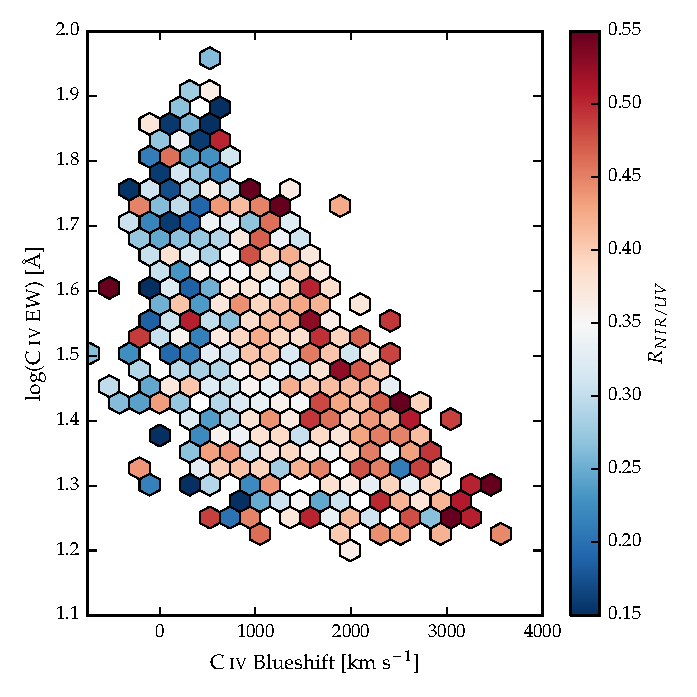
\includegraphics[width=\columnwidth]{figures/chapter05/hot_dust_ratio.pdf}
  \caption[{Hot dust abundance as a function of rest-frame EQW and blueshift of the \ion{C}{IV} line.}]{Rest-frame EQW and blueshift of the \ion{C}{IV} line for 7,115 SDSS DR7 quasars. The colours of the hexagons denote the median hot dust (T$\simeq$1200\,K) abundance for all quasars at a given EQW and blueshift. Quasars with the most extreme outflow signatures are predominantly hot-dust rich. Only bins containing a minimum of two objects are plotted.}
  \label{fig:civ_hot_dust}
\end{figure}

\begin{figure}
\centering
  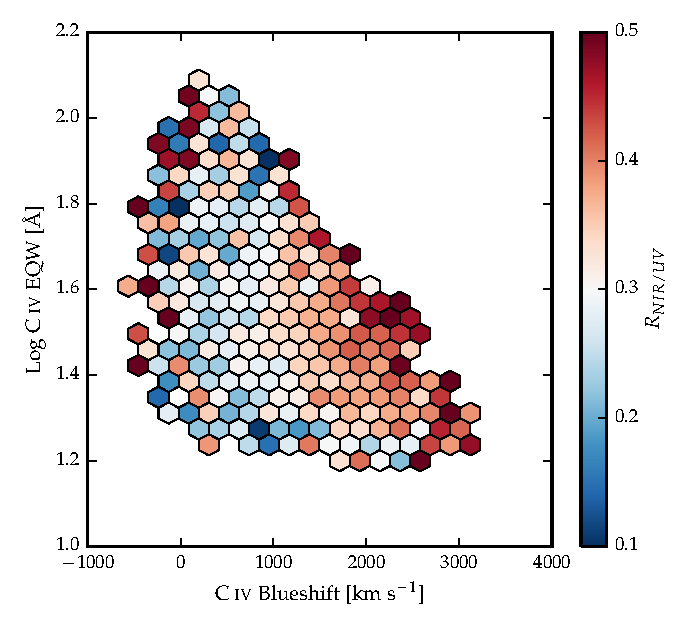
\includegraphics[width=\columnwidth]{figures/chapter05/hot_dust_beta.pdf}
\caption[{Hot dust abundance as a function of rest-frame EQW and blueshift of the \ion{C}{IV} line.}]{Rest-frame EQWand blueshift of the \ion{C}{IV} line for 7,115 SDSS DR7 quasars. The colours of the hexagons denote the median hot dust (T$\simeq$1200\,K) abundance for all quasars at a given EQW and blueshift. Quasars with the most extreme outflow signatures are predominantly hot-dust rich. Only bins containing a minimum of two objects are plotted. \todoinline{Change hot dust abundance.}}
  \label{fig:hot_dust_beta}
\end{figure}

\begin{figure}
\centering
  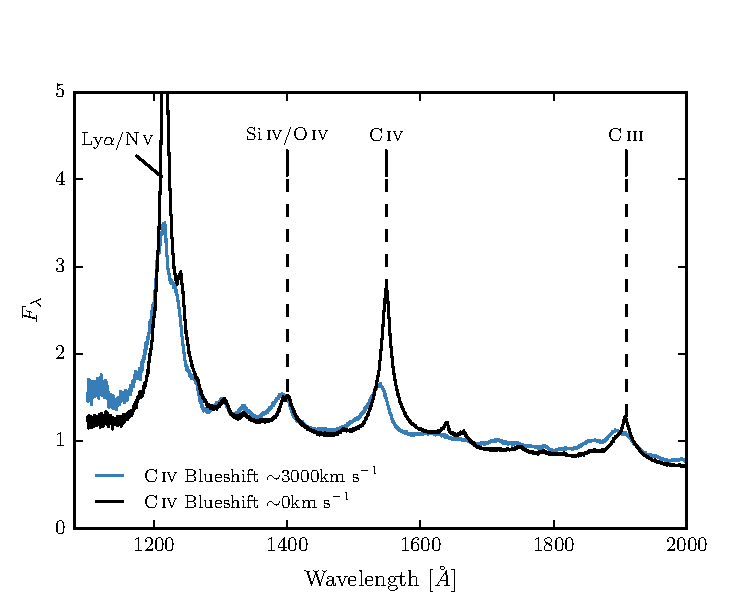
\includegraphics[width=\columnwidth]{figures/chapter05/blueshift_composite.pdf}
\caption{}
  \label{fig:blueshift_composite}
\end{figure}

\section{Discussion}

\citet{roseboom13} studied a similar sample of luminous type 1 quasars. 
They, like us, modelled the NIR emission using a blackbody and modelled the emission at longer wavelengths using a clumpy torus model. 
They find that while $L_{1-5\mu m}$/$L_{IR}$ appears relatively insensitive to $L_{bol}$ and $L_{IR}$, a strong correlation appears between $L_{1-5\mu m}$/$L_{IR}$ and $L_{IR}/L_{bol}$ (i.e. the dust covering factor). 
They explain this correlation by postulating that as the covering factor of the torus decreases, the maximum inclination at which a type 1 quasar would be seen increases. 
An increase in the inclination will mean direct sight lines to more of the inner wall of obscuring material closest to the accretion disc.

\citet{mor11} also looked at the hot dust properties of a sample of $0.75 < z < 2$ quasars, with photometry from SDSS and WISE. 
They modelled the NIR emission with hot clouds of pure graphite dust. 
They reported an anti-correlation between the covering factor of hot dust clouds and the quasar bolometric luminosity. 
Like us, they neglect cooler dust components which will dominate the SED at longer wavelengths. 
As we have discovered (see Figure residual plot), the missing flux decreases with redshift because we observe shorter rest-frame wavelengths when the observed spectrum is redshifted to a greater degree. 
This will induce an anti-correlation between the luminosity of the hot dust component and the luminosity of the quasar (which is correlated with redshift). 
At z=0.75, the $W3$ band-pass (the longest in their fits) is sensitive to flux from 6.9$\mu$m; at this wavelength we expect the contribution from cooler dust to dominate over the hot dust. 
It is possible that this effect could explain the tension with our own result that $R_{NIR/UV}$ does not depend on the quasar luminosity in our low-$z$ sample. 

\citet{shen14} quantify the relative torus emission using the $r-W1$ colour for a sample of $0.4 < z < 0.8$ SDSS quasars. 
At these redshifts $W1$ is observing between 1.9 and 2.4 microns in the rest-frame of the quasar, which suggests that they are sensitive to the same component of hot dust which we are investigating. 
They observe a mild trend of decreasing relative torus emission as the quasar luminosity increases. 
We note that their use of the $r-W1$ at much higher redshifts may be problematic, as the $W1$ flux will be increasingly dominated by direct emission from the accretion disc. 

\citet{gallagher07} undertook a similar investigation for a much smaller sample of 234 radio-quiet quasars.

Reverberation measurements of nearby AGNs suggest the NIR emission is dominated by hot dust very close to the central source \citep[few tens of light days; e.g.][]{minezaki04,suganuma06}. 
The hot dust signature could contain information about inner face of an obscuring torus structure and/or constrain the dust content of an accretion disc wind. 
Several studies have shown that the luminosity of the NIR excess emission correlates with that of the central engine with a slope close to unity \cite[e.g.][]{gallagher07}, suggesting that the dust is reprocessing radiation from the accretion disc. 

Outflows may emerge from the outer region of the accretion disc or even the innermost region of the torus, in which the gas clouds are dusty and relatively cold.  
Indeed, there is observational evidence for dusty outflows close to the central engine \citep[e.g.][]{bowler14}.
\todo{Paul: yes, but not very dusty in context of cold dusty clouds, $\sim$ 0.01 mag per `cloud'.}
The dust is heated by the central engine, and radiates in the NIR band. 
\citet{wang13}, fitting the NIR emission with a single power-law, found that objects with strong outflow signatures (blue-shifted \ion{C}{IV}) have more hot dust emission relative to the accretion disc emission in a large sample of $z\sim2$ non-BAL quasars. 
It could be that this correlation is induced by a third factor that simultaneously affects outflows and dust emission, for instance the inclination angle or metallicity. 
Alternatively the dust could be intrinsic to outflows and may have a non-trivial contribution to the outflow acceleration \citep[e.g.][]{fabian12}. 
Also found by \citet{shen14}. 

Several other investigations have drawn attention to the rest-frame NIR SEDs, with populations of `dust free' objects postulated \citep{hao10,hao11,jiang10,mor11} 


\subsection{Eddington ratio}

Wang et al., Zhang et al., and Mor \& Trakhtenbrot find no significant dependence of the amount of hot dust on the Eddington ratio. 
Is this because the Eddington ratio is wrong or because it's more complicated? (can high accretion objects with no evidence for strong outflows.)

\subsection{Spectral properties}

In the dusty wind model - first proposed by \citet{konigl94} and later developed by, amongst others, \citet{everett05}, \citet{elitzur06}, \citet{keating12} - the `torus' is the dusty part of a magneto-hydrodynamic wind beyond the dust sublimation radius. 
The MHD wind is roughly polar, and so the hot dust forms a vertical `wall' around the accretion disc.  
UV photons from the accretion disc accelerate the wind via radiation line driving. 
That flattens the geometry of the wind and exposes more surface area that is viewable on a relatively face-on line of sight.  
The radiation pressure is increased at higher luminosities and/or accretion rates.
This can flatten the geometry of the wind, thereby increasing the range of angles for which the inner edge of the dusty wind - where dust is at it's sublimation temperature - can be observed. 
A direct prediction is therefore that the in a quasars with high accretion rates and strong outflows, the emission from hot dust should be enhanced. 


\section{Further work}

What more is needed to test model(s)?  

\subsection{Hot-Dust-Poor Quasars}

The near-IR emission from AGN is generally explained by thermal emission from dust grains at the edge of the dusty torus closest to the accretion disk. 
The dust is heated to its sublimation temperature \citep[1300-2000K][]{barvainis92} by emission from the accretion disc. However, \citet{hao10} reported that 6\% (at $z \lesssim 2$) to 20\% (at $2 \lesssim z \lesssim 3.5$) of the quasars in the X-ray selected XMM-COSMOS Type 1 AGN sample \citep{brusa10} have an unusually small amount of hot dust emission, despite having normal accretion disc spectra. 
They infer a torus covering factor of  $\sim$2\% to 30\% for these `hot dust poor' (HDP) quasars, well below the $\sim$75\% predicted by unified models \citep[e.g.][]{krolik88}. 
\citet{hao11} found that HDP quasars were just as common in the \citet{richards06} Spitzer/SDSS sample ($8.7\% \pm 2.2\%$) and the \citet{elvis94} Palomar-Green-quasar-dominated sample ($9.5\% \pm 5.0\%$). 
Either the hot dust is destroyed (dynamically or by radiation), or the dust is not centred on the SMBH, which could happen during a major merger \citep[e.g.][]{blecha11}. 
Alternatively, misaligned accretion disks, which will result from discrete isotropic accretion events \citep{volonteri07}, will lead to a wider range of covering factors \citep{lawrence10}. 

At higher redshifts, \citet{jiang10} found two HDP quasars in a sample of 21 at $z\sim6$. 
They find that at $z\sim6$ the hot dust abundance is roughly proportional to the black hole mass, indicating that the two grow at about the same rate. 
The two HDP quasars also have the smallest SMBH masses, and may be too young to have formed a significant amount of hot dust.
